\lhead{\emph{Arquitectura software}}
\chapter{Arquitectura software}

Con el objetivo de facilitar la comprensión del sistema como un todo esta memoria se estructura partiendo de los cimientos del sistema, ascendiendo hasta las aplicaciones de más alto nivel manipuladas por los usuarios, describiendo de forma exhaustiva todos los aspectos de relevancia y esfuerzos llevados a cabo para diseñar y desarrollar cada uno de los componentes del sistema.

\section{Sistema operativo}

Una pieza fundamental del \textit{software} del sistema es la capa más básica del mismo, el sistema operativo. Es por ello clave elegir un sistema adecuado para los objetivos que se desean alcanzar.

Como se describió en \ref{problema:sistemaoperativo}, se utilizará el sistema operativo Arch Linux en su variante para procesadores ARM por su diseño altamente modular, eficiencia y capacidad de adaptabilidad. Sobre dicho sistema operativo se desarrollarán el resto de componentes, sin que ello implique un diseño adaptado a este sistema operativo.

\subsection{Características técnicas de Arch Linux}
\label{archlinux:description}

\textbf{Arch Linux} es una distribución del sistema operativo GNU/Linux creada y mantenida por una comunidad de usuarios. Desarrollada de forma independiente, es lo suficientemente versátil como para satisfacer cualquier propósito. Su desarrollo se centra en la simplicidad, elegancia y minimalismo, asumiendo que el usuario añadirá los componentes que restan para conseguir el entorno que desee. Dicho minimalismo se traduce en una arquitectura basada en paquetes que conforman en su conjunto un sistema fácil de comprender por el usuario, y que cuentan con una gran cantidad de documentación fácilmente accesible. La consecuencia directa de este minimalismo es el rendimiento del sistema. Una instalación de Arch Linux se limita al conjunto de paquetes mínimo para contar con un sistema completamente funcional, delegando al usuario la adición de nuevos paquetes. Este enfoque permite optimizar de forma sencilla el rendimiento del sistema, al no contar con paquetes innecesarios.

Arch Linux está basado en un modelo de liberación continua (\textit{rolling release}) lo cual significa que el sistema está en constante desarrollo (en contraste con un sistema de versiones). El \textit{software} se actualiza de forma continua, siendo únicamente necesario realizar una actualización de los paquetes que conforman el sistema para contar con la última versión. Este modelo de desarrollo permite contar con las últimas versiones del software incluido de forma casi inmediata a su liberación. Generalmente los paquetes que se incluyen sin modificaciones por parte del proyecto (esta práctica se denomina \textit{upstream}, pues la fuente del software es el propio autor del mismo), tal y como el fueron creados para su uso.

La gestión de paquetes se realiza utilizando la herramienta \textbf{pacman}\cite{pacman}, creada por y para el proyecto. El repositorio oficial ofrece una gran cantidad de paquetes, si bien su tamaño es significativamente inferior al \textit{Arch User Repository} (AUR), que contiene paquetes creados y mantenidos por usuarios.

Arch Linux utiliza el sistema de arranque \textbf{systemd}\cite{systemd}, un conjunto de módulos que proporcionan una gestión de dependencias entre servicios del sistema más eficiente y sencilla que el cargador clásico de las distribuiciones GNU, \textbf{init}\cite{init}, inspirado en el utilizado por UNIX System V.

Otro de los aspectos de relevancia del sistema es la comunidad creada alrededor del mismo, que fomenta la implicación de cualquier usuario en cualquiera de los aspectos de relevancia en el desarollo del sistema. La documentación del sistema es extensa y cuenta con recursos tanto para las características propias del sistema como para herramientas de terceros utilizadas en el mismo. %Además, la comunidad de Arch Linux es famosa por la gran y exhaustiva cantidad de documentación que mantiene, así como las diferentes opciones de soporte a cualquier nivel que ofrece a través de diferentes canales\citationneeded.

Dichos aspectos del proyecto y una serie de consideraciones adicionales se recogen en los preceptos definidos en el documento \textit{The Arch Way}\cite{thearchway}, inspirado en el principio de desarrollo \textbf{KISS} (\textit{Keep It Simple, Stupid}), muy popular en el entorno de los sistemas operativos UNIX.\citationneeded{http://people.apache.org/~fhanik/kiss.html}. 

Arch Linux ARM\citationneeded[http://archlinuxarm.org/] es un proyecto derivado de Arch Linux que tiene como objetivo portar el sistema operativo a dispositivos basados en la arquitectura ARM (pues el proyecto raíz está enfocado únicamente en las arquitecturas i686 y x68\_64), generalmente sistemas embebidos, habiendo conseguido la compatibilidad con las versiones v5te, v6h y v7h de la arquitectura. El proyecto mantiene la misma filosofía de diseño que su progenitor, siendo el buen rendimiento del sistema operativo uno de los aspectos que propician el uso de esta distribución en sistemas con un capacidad de cómputo reducida. Es una de las principales opciones a la hora de realizar proyectos con este tipo de computadores\cite{distrowatch:arm}.%TODO: Revisar



%Además, Arch Linux apuesta por un modelo de desarrollo de liberación continua (\textit{rolling releases}). El sistema operativo no se distribuye en versiones, sino en imágenes con las últimas versiones de los paquetes disponibles, lo cual posibilita contar con las últimas versiones de las herramientas presentes en el sistema operativo poco tiempo (o de forma inmediata) a su liberación. El modelo de desarrollo sigue este principio de forma tan estricta, que basta una actualización de todos los paquetes del sistema mediante el gestor propio de la distribución (\textbf{pacman}) para actualizar el sistema operativo (en contraste con operaciones específicas para este cometido, como ocurre con otros sistemas operativos).

%El sistema operativo delega la responsabilidad del mantenimiento de todos los componentes al usuario en un grado mayor que el que pueden ofrecer otras distribuciones. Esto permite a los usuarios contar con completa libertad para modificar componentes del sistema en función de sus intereses a cualquier nivel\citationneeded{https://wiki.archlinux.org/index.php/The\_Arch\_Way}.


El proceso de elección del sistema operativo puede observarse en \ref{os:evaluation}.


\subsection{Sistema operativo en el servidor}

En el caso del servidor que provee diferentes servicios de apoyo a los nodos principales (ver \ref{sistema:arquitectura}) se utiliza el sistema operativo Debian GNU/Linux. Este sistema operativo tiene como objetivo la estabilidad del sistema en detrimento de las últimas características del \textit{software} que lo conforma.

\section{Servicios integrados en el sistema operativo}

Diversos componentes del sistema operativo son utilizados para llevar a cabo operaciones de gestión o como herramienta para la creación de aplicaciones en niveles superiores. Gracias a la integración de estos componentes en niveles inferiores, es posible ofrecer dichos servicios a cualquier aplicación de usuario. 


\subsection{Gestión de servicios}

\textbf{systemd} es utilizado como gestor de los diferentes servicios del sistema, así como aquellos creados en el proceso de desarrollo del mismo. Se aprovecha su capacidad para gestionar dependencias entre los diferentes componentes (orden de arranque, qué servicios deben arrancarse para que otros puedan funcionar\dots) para establecer el orden de inicio al arrancar el sistema o iniciar automáticamente servicios sobre los que dependan otros.

\textbf{systemd} define cada uno de los diferentes servicios (``unidades'') en un fichero independiente.

\section{Descubrimiento de servicios}

Uno de los problemas típicos a la hora de crear un sistema distribuido es la localización de cada uno de los nodos que lo conforman. Al no existir un coordinador, es difícil establecer un mecanismo de interconexión entre los diferentes nodos que sea escalable e independiente de factores externos (e.g. IP asignada en un momento dado, número de nodos en la red).


Soluciones como el uso de servidores de nombres (\textbf{DNS}) permiten crear estructuras jerárquicas donde cada nodo está identificado por un nombre previamente asignado y conocido. Como primera propuesta de solución se plantea el uso de los nombres de equipo que el servidor \textbf{DHCP} presente en la infraestructura otorga. Con esta solución los nodos serían accesibles mediante un identificador invariable en el tiempo (en contraste con una IP dinámica). Sin embargo, dicha solución presenta un grave problema en materia de escalabilidad: no existe un ``directorio'' que recoja qué nodos están activos en un momento dado ni que refleje adiciones en la lista original de nodos, por lo que para poder realizar cualquier cambio en el conjunto de nodos del sistema será necesario configurar cada equipo manualmente. También existen protocolos inspirados en enfoque como \textbf{mDNS} (\textit{Multicast Domain Name Service}) donde la necesidad de un servidor de nombres desaparece, y los nodos son capaces de realizar el descubrimiento mediante mensajes uno-a-muchos\cite{rfc6762}. Implementaciones de este protocolo, como \textit{Bonjour}, \textit{Avahi} o \textit{AppleTalk} (ya descontinuado) han sido evaluadas a la hora de buscar una solución a este problema. Sin embargo, estas y otras soluciones similares no responden a una de las necesidades básicas del sistema a construir: la condición de que la información que conoce cada nodo sobre el resto en el arranque del sistema es nula. Si bien con \textbf{mDNS} desaparece la necesidad con un servidor de nombres y es posible realizar operaciones de descubrimiento de servicios, este y otros protocolos similares asumen que la información de un nodo presente de una red local es de interés para el resto de miembros de la misma, lo cual dificulta la independencia de un conjunto de equipos frente al resto en el mismo espacio de direcciones.

%Avahi?

\subsection{MarcoPolo, el protocolo de descubrimiento de servicios}
\label{marcopolo}

Una de las características clave del sistema consiste en la escalabilidad del mismo en tiempo de ejecución: no es necesario conocer qué nodos participan en el sistema hasta que no se requiera de los mismos. Además, se pretende optimizar al máximo cada uno de los nodos del sistema por separado, por lo que designar a uno de ellos como ``autoridad'' frente a la que el resto de nodos se registren y esta actúe posteriormente como coordinador y \textit{``resolver''} supone una dedicación de recursos innecesaria y que dificulta la escalabilidad del sistema. Además, la gestión del espacio de direcciones de la red en la que se integra el sistema, que es compartido con una gran cantidad de equipos adicionales, no recaería en dicho coordinador. Esto implica que las direcciones de cada nodo son asignadas por un servidor DHCP sobre el que no se tiene control y cuyas asignaciones son dadas por intervalos de tiempo pequeños\footnote{Durante el desarrollo del sistema se observa que las direcciones son asignadas por periodos de tiempo pequeños y no suelen repetirse a menos que dicha dirección no haya sido asignada anteriormente, fenómeno que suele darse con bastante frecuencia.}. %TODOEsto implica que no es posible contar con un nodo coordinador sin un espacio de nombres anteriormente definido.
Por otro lado, la clave de este sistema no la constituye la disponibilidad de un nodo, sino las aplicaciones distribuidas que pueden utilizarse en el mismo (de ahora en adelante serán denominadas ``servicios''). Un nodo puede contar con un conjunto de servicios diferente al de sus vecinos, y por tanto colaborará en unas tareas y en otras no en virtud de dicha disponibilidad.%TODO Este requisito no es satisfecho por la mayoría de los sistemas anteriormente mencionados.

Motivada por esta serie de características surge la necesidad de crear un protocolo de descubrimiento de nodos y servicios basado principalmente en los servicios que dichos nodos pueden (y desean) ofrecer. Además, siendo uno de los objetivos funcionales del sistema el aprovechamiento del mismo como herramienta didáctica, surge la necesidad de que dos conjuntos de nodos puedan trabajar en la misma red de forma independiente. Como aproximación para satisfacer estas necesidades surge el procolo de descubrimiento de servicios \textbf{MarcoPolo}.

\subsubsection{Introducción}

\textbf{MarcoPolo} es un protocolo de descubrimiento de servicios cuya dinámica y nombre se inspiran en el juego homónimo\citationneeded[\href{http://en.wikipedia.org/wiki/Marco\_Polo\_\%28game\%29\#cite\_note-play-1.http://www.wisegeek.com/what-is-the-game-marco-polo.htm}{http://en.wikipedia.org/wiki/Marco\_Polo\_\%28game\%29\#cite\_note-play-1.http://www.wisegeek.com/what-is-the-game-marco-polo.htm}], en el cual uno de los integrantes debe encontrar al resto privado de visión mediante ecolocalización (gritando la palabra clave ``Marco'', cuya respuesta por parte del resto de jugadores es ``Polo''). El protocolo se compone de dos roles claramente diferenciados (e independientes aún siendo ejecutados en el mismo nodo): \textbf{Marco}, encargado de enviar consultas a la red y \textbf{Polo}, que emite una respuesta a dichos comandos y gestiona la información de cada nodo. %TODO: 

Con el objetivo de posibilitar la coexistencia de varias ``mallas'' de nodos independientes (donde los servicios ofrecidos por un nodo sean conocidos y consecuentemente aprovechables únicamente por el resto) a la vez que las consultas son realizadas a todos los integrantes sin necesidad de conocer su identificador en la red (dirección a nivel de red o enlace, nombre \textbf{DNS}) se utilizan mensajes uno-a-muchos, conocidos con el nombre \textit{multicast}, donde cada una de las ``mallas'' se comunicará con el resto de integrantes de la misma a través de un grupo preestablecido (o consensuado por dichos nodos).

\subsubsection{Funcionamiento}

El protocolo se basa en el envío de mensajes a un grupo multicast acordado previamente (existiendo un grupo designado por defecto). Los nodos suscritos a dicho grupo recibirán dicho mensaje y lo procesarán, emitiendo una respuesta dirigida únicamente al nodo que ha realizado la solicitud en caso de que el mensaje solicite un servicio que el nodo ofrezca. En caso contrario no se emitirá ninguna respuesta. Dicho mensaje incluirá información adicional, como el método de acceso al servicio, estado del nodo, etcétera.

El solicitante esperará durante un tiempo pequeño a que haya respuesta por parte del resto de nodos, recogiendo todos los mensajes recibidos. Una vez que el tiempo de espera haya pasado, se retornarán los resultados al programa o usuario solicitante.

\subsection{Comandos}

Los mensajes utilizados se denominan \textit{comandos} y contienen las consultas sobre un servicio, nodo o información sobre la propia \textit{malla} que se desea conocer, así como la respuesta a dichas consultas. Dichos comandos son enviados como cadenas de texto que almacenan la información en estructuras de datos JSON (\textit{JavaScript Object Notation}) debido a la gran legibilidad de estas por humanos y máquinas, y la popularidad de este formato como mecanismo de transmisión de informaciónla gran cantidad de herramientas disponibles para su creación y procesado.

Los comandos de MarcoPolo constituyen las primitivas del protocolo. Actualmente se cuenta con las siguientes primitivas y las correspondientes respuestas:
\begin{landscape}
\begin{table}[H]
\begin{tabular}{|p{2.35cm}|p{1.2cm}|p{4.5cm}|p{5cm}|p{5cm}|p{3.5cm}|}
\hline
\textbf{Nombre} & \textbf{Emisor} & \textbf{Función} & \textbf{Información} & \textbf{Respuesta esperada} & \textbf{Protocolo}\\ \hline

\textbf{Marco} & Marco & Descubrir todos los nodos presentes en la malla & Únicamente se incluye el nombre del comando & Un comando \textit{Polo} por cada nodo disponible en la red o ninguna si no existe ningún nodo. & UDP \textit{multicast} al puerto 1338.\\ \hline

\textbf{Polo} & Polo & Notificar de la presencia de este nodo al recibir un mensaje \textbf{marco} & Información opcional sobre el nodo (e.g. estado, \textit{hostname}\dots), incluyendo opcionalmente información adicional  & Ninguna &  UDP \textit{unicast} al puerto efímero del nodo solicitante.\\ \hline

\textbf{Request-For} & Marco & Conocer todos los nodos que ofrecen un servicio a través de su identificador único en el sistema & Identificador del servicio a descubrir & Un mensaje \textit{OK} con información opcional sobre el nodo o el servicio & UDP \textit{multicast} al puerto 1338.\\ \hline

\textbf{OK} & Polo & Comando utilizado para emitir una respuesta a una petición. & Respuesta a un comando con la información solicitada & Ninguna & UDP \textit{unicast} al puerto efímero de la pregunta.\\ \hline

\textbf{Services} & Marco & Descubrir todos los servicios ofrecidos por un nodo & No se envía información adicional con el comando & \textbf{OK} con una lista de los identificadores del servicio o ninguna si el nodo no se encuentra activo. & UDP \textit{unicast} al puerto 1338.\\ \hline
\end{tabular}
\caption{Comandos del protocolo MarcoPolo}
\end{table}
\end{landscape}

\subsection{Esquemas de comunicación}

\subsubsection{Comando \textbf{Marco}}

%TODO \begin{figure}[H]
% \centering
% 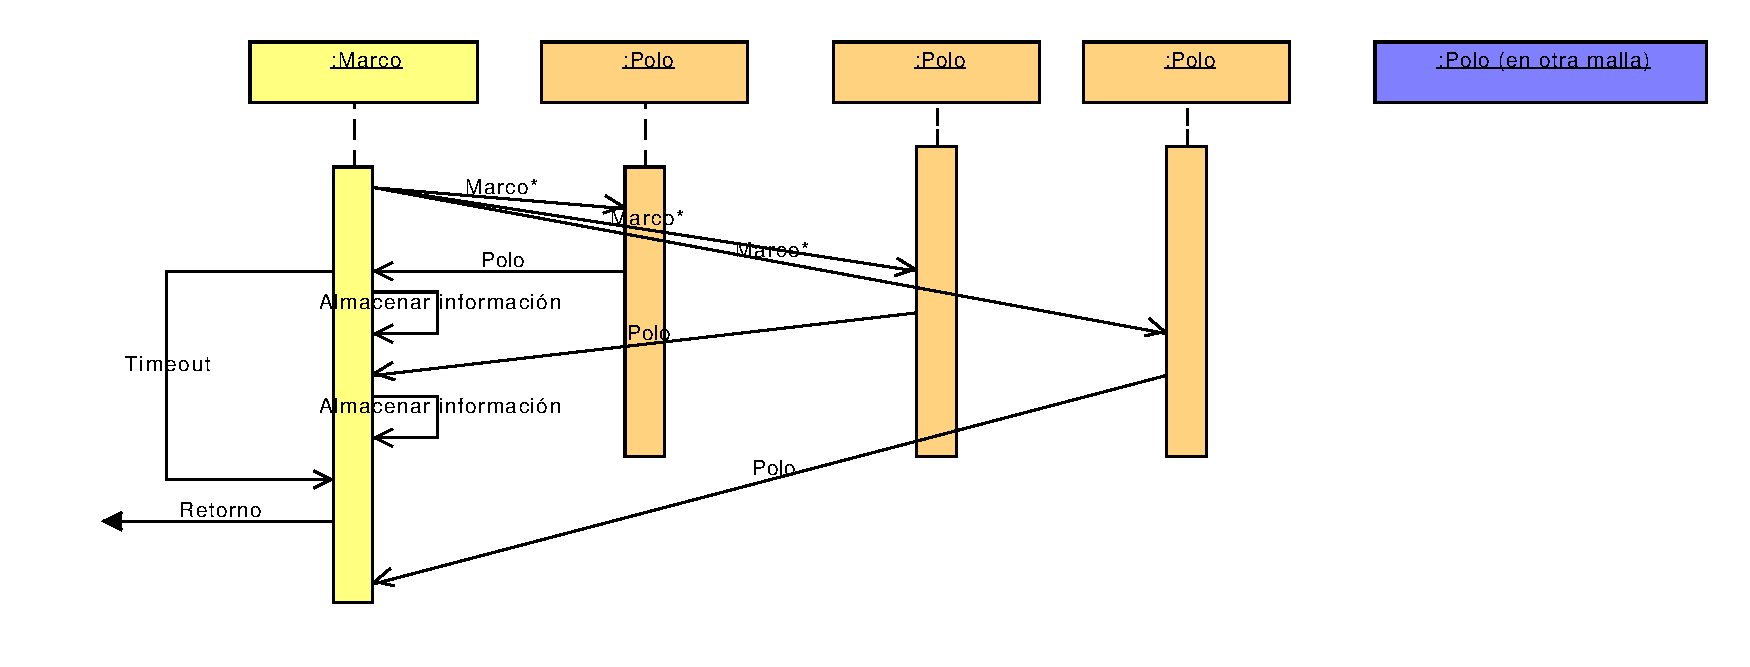
\includegraphics[width=\textwidth]{Diagrams/Sequence/marcocompleto}
% \caption[Interacción al enviar el comando \textbf{Marco}]{Interacción al enviar el comando \textbf{Marco}. Los mensajes a grupos \textit{multicast} se indican con ``*''}
% \label{fig:secuencia_marco}
% \end{figure}

El comando Marco se envía al grupo \textit{multicast} definido en la configuración de la instancia local de \textbf{Marco} o a aquel definido en tiempo de ejecución. Los nodos suscritos a dicho grupo (aquellos que pertenecen a la malla) reciben el mensaje y emiten una respuesta \textbf{Polo}. Debido a la falta de una conexión entre los nodos (todos los mensajes son intercambiados utilizando el protocolo \textbf{UDP}) se fija un tiempo de espera, durante el cual se reciben y acumulan todas las respuestas. Al pasar dicho tiempo, se retornan los resultados y los mensajes recibidos posteriormente son ignorados.

% TODO\begin{figure}[H]
% 	\centering
% 	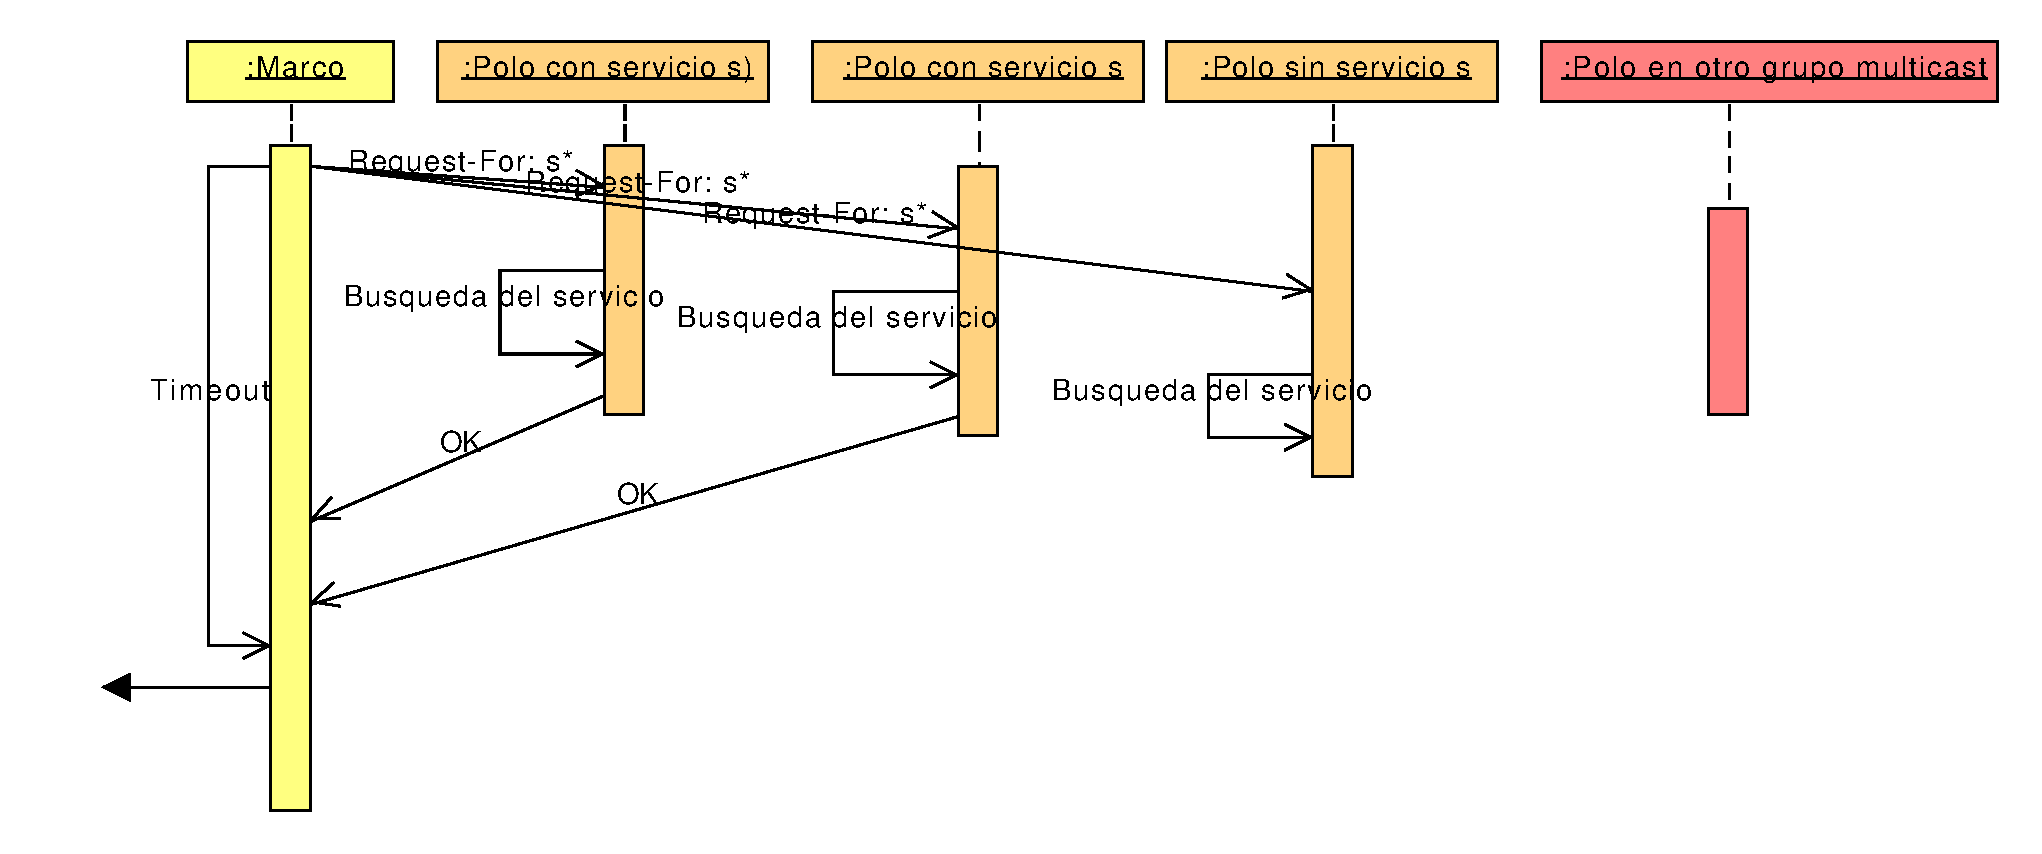
\includegraphics[width=\textwidth]{Diagrams/Sequence/request_for}
% 	\caption[Interacción al enviar el comando \textbf{Request-For}]{Diagrama de interacción al enviar el comando \textbf{Request-For}. Los nodos comprueban si deben ofrecer el servicio identificado por la clave \textit{s}. En caso de que la búsqueda sea exitosa se retorna un mensaje indicando la disponibilidad de dicho nodo. En caso contrario no habrá respuesta alguna.
% 	Los mensajes enviados a grupos \textit{multicast} se indican con ``*''}
% 	\label{fig:secuencia_request_for}
% \end{figure}

% TODO\begin{figure}[H]
% 	\centering
% 	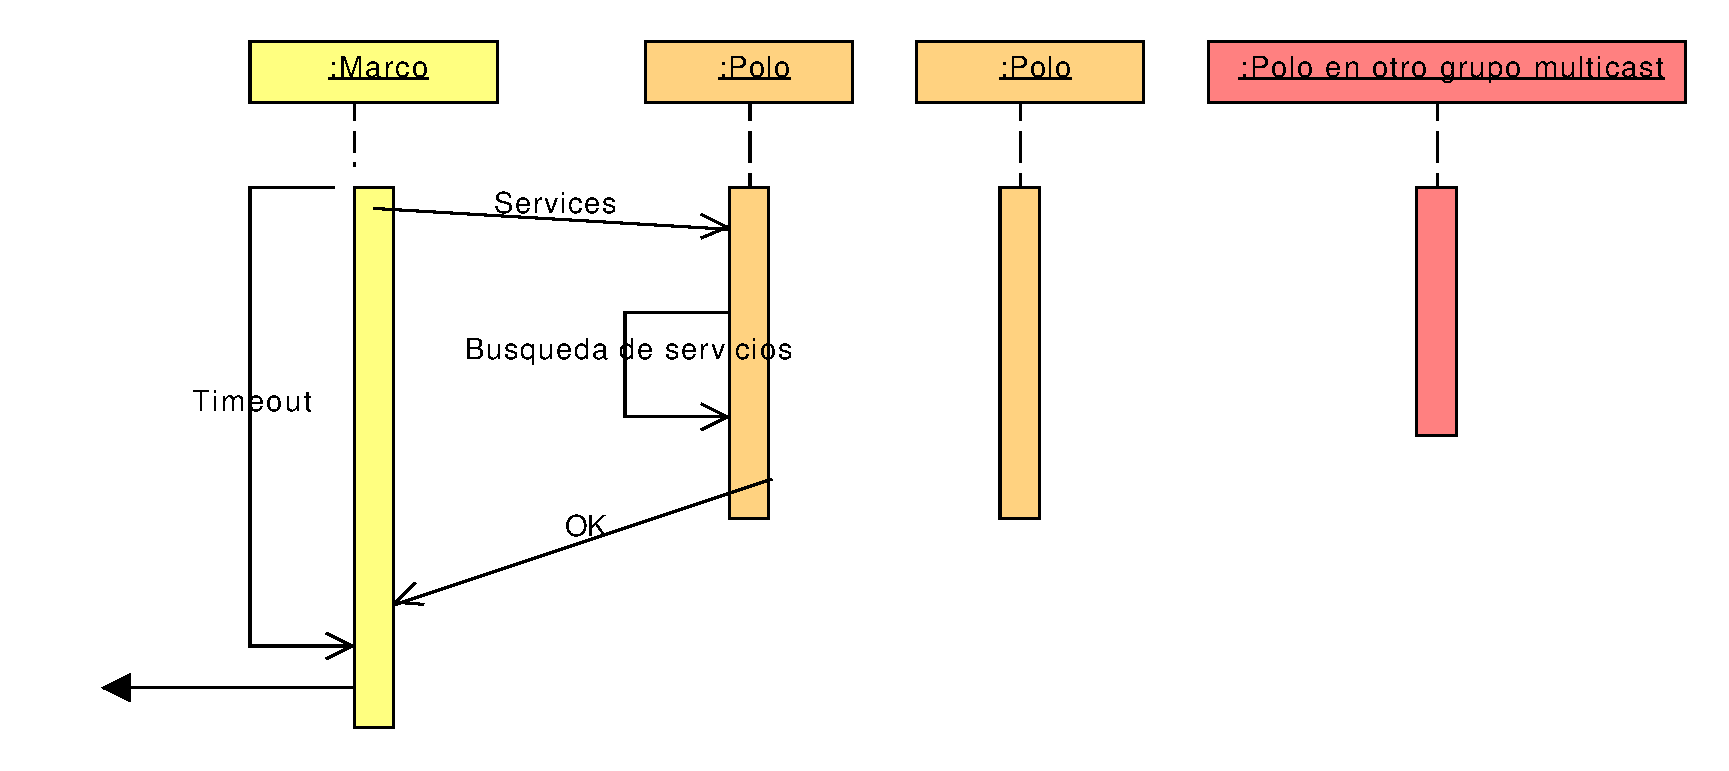
\includegraphics[width=\textwidth]{Diagrams/Sequence/services}
% 	\caption[Diagrama de interacción al enviar el comando \textbf{Services}]{Diagrama de interacción al enviar el comando \textbf{Services}. El nodo al que se le envía el comando consulta la información sobre los servicios que posee y posteriormente envía una respuesta a la instancia de Marco que ha realizado la consulta. Obsérvese toda la información es enviada en modo \textit{unicast}}
% 	\label{fig:secuencia_services}
% \end{figure}

\subsection{Arquitectura en detalle}

La funcionalidad del protocolo se segmenta en dos roles claramente definidos e identificados: \textbf{Marco} y \textbf{Polo}. Dicha funcionalidad se implementa en dos ejecutables completamente independientes, que pueden por tanto coexistir o ser ejecutados sin presencia del otro.

Estos ejecutables están diseñados para ser iniciados al arranque el equipo, aprovechando para ello las herramientas que el este provee\footnote{Los ejecutables han sido configurados para ser compatibles con los gestores de arranque \textbf{init} y el más reciente \textbf{systemd}.}, y se ejecutan en segundo plano de forma continua (es por ello pueden ser categorizados como procesos \textit{daemon}).

Toda la funcionalidad se ejecuta en un único proceso que se encarga de la creación de los diferentes canales de comunicación (utilizando la API de \textit{sockets} de Berkeley). Dichos canales de comunicación son gestionados por la utilidad \textbf{Twisted}\citationneeded, que simplifica el trabajo con la API, en particular a la hora de crear \textit{sockets} asíncronos.

\subsubsection{Configuración}

Todos los aspectos modificables de cada rol, tales como el grupo \textit{multicast} al que suscribirse o el tiempo de espera predeterminado se definen en un archivo de configuración alojado en el directorio \texttt{/etc/marcopolo} (siguiendo la estructura definida en el \textit{Filesystem Hierarchy Standard} \cite{fhs}).

% \begin{figure}[H]
% 	\centering
% 	\VerbatimInput{/home/martin/TFG/Documentación/memoria-tfg/memoria/Code/confdir.txt} %TODO
% 	\caption{Árbol de directorios dentro del directorio de configuración}
% 	\label{fig:arbol_marcopoloconf}
% \end{figure}

Los archivos de configuración de cada uno de los \textit{daemons} sigue la típica estructura clave-valor presente en archivos de configuración de servicios del sistema. Por el contrario, la información de los servicios a ofrecer sigue la sintaxis de un fichero \textbf{JSON}\footnote{La razón de esta decisión de diseño es la facilidad de interpretación de dicho formato y la legibilidad que ofrecen.}. Todos estos ficheros son leídos al arrancar el ejecutable, y su modificación no tendrá efectos hasta la próxima vez que se inicie el servicio.%TODO (salvo excepciones que veremos a continuación).

\javascriptcode{statusmonitor}{Un archivo que describe el servicio status monitor}{1}{7}

\subsubsection{Archivos auxiliares}

\paragraph{Log}
Toda la información sobre la ejecución de los \textit{daemons} se refleja en los archivos de \textit{log} presentes en el directorio \texttt{/var/log/marcopolo}. El nivel de log se configura en el parámetro \texttt{LOGLEVEL} de cada uno de los \textit{daemons} y puede tomar uno de los siguientes valores:

\begin{itemize}
\item \textbf{Error} Errores internos durante la ejecución.
\item \textbf{Warn} Advertencias sobre posibles situaciones atípicas.
\item \textbf{Info} Información de interés sobre el funcionamiento del sistema.
\item \textbf{Debug} Información de depuración.
\end{itemize}

%\logcode{/home/martin/TFG/Documentación/memoria-tfg/memoria/Code/marcod}{Caption}{1}{3} %TODO

\paragraph{Registro de ejecución}

En ocasiones es necesario conocer el identificador del proceso \textbf{PID} del \textit{daemon}. Para ello se almacena en el directorio \texttt{/var/run/(marcod.pid|polod.pid)} dicho identificador, que puede ser aprovechado por el gestor de arranque del proceso.

\subsection{Integración de los \textit{daemons} en el sistema operativo}

Los \textit{daemons} se integran en el arranque del sistema a través de los ficheros de configuración de \texttt{init}\citationneeded{} o \texttt{systemd} dependiendo del gestor disponible en el sistema operativo sobre el que se ejecuten los procesos. Por defecto los \textit{daemons} se ejecutan durante todo el ciclo de vida del computador, pero pueden ser reiniciados o detenidos arbitrariamente por voluntad del administrador.

% TODO: para el documento en detalle \begin{lstlisting}
% systemctl start (marco|polo)
% systemctl stop (marco|polo)
% systemctl restart (marco|polo)
% systemctl reload polo #Orden exclusiva de Polo
% \end{lstlisting}

% El comando \texttt{reload} permite actualizar la lista de servicios que \textbf{Polo} ofrece sin tener que detener todo el proceso para ello. Dicho comportamiento se consigue de forma similar al comando \texttt{reload} de Apache, enviando la señal \texttt{SIGUSR1} al proceso. 

\subsection{Conexiones con MarcoPolo}

La funcionalidad de \textbf{MarcoPolo} no se limita al descubrimiento de los servicios del sistema, por lo que es necesario ofrecer a los usuarios del clúster herramientas que permitan integrar sus aplicaciones distribuidas con estos servicios. Dichas herramientas, conocidas como \textit{bindings}, permiten exponer públicamente la funcionalidad de \textbf{MarcoPolo} para que pueda ser aprovechada por otros usuarios.

Se han creado \textit{bindings} para los lenguajes de programación \textbf{C}, \textbf{C++}, \textbf{Python} y \textbf{Java}. Todos ellos son consistentes entre sí, manteniendo la misma sintaxis para realizar el mismo tipo de operación a la vez que aprovechan las características propias de cada lenguaje. Dicha filosofía está inspirada en el funcionamiento de las primitivas de la API de resolución de nombres en red (\texttt{netdb.h})\cite{netdb}, por lo que los \texttt{bindings} se comunican con la instancia local de Marco o Polo a través de \textit{sockets} vinculados a la dirección IP local (127.0.1.1).

Todos los \textit{bindings} deben implementar el mismo conjunto de primitivas, definidas en la documentación de refencia de MarcoPolo (ver anexo). La mayoría de primitivas tienen como objetivo el descubrimiento y publicación de servicios. Sin embargo, varias de ellas permiten realizar consultas sobre la información del propio nodo y se plantea la creación de más primitivas que sigan dicha filosofía

%TODO \paragraph{Primitivas en el \textit{binding} de Marco}
% \begin{itemize}
% \item \texttt{request\_for(service, timeout=None)}
% Retorna una lista de nodos que ofrecen el servicio indicado en \texttt{service}. Esta función bloquea la ejecución del proceso hasta que el tiempo de espera de nuevas respuestas se cumple (si bien esto no constituye un problema para la mayoría de aplicaciones, es importante que sea conocido por el programador). Si se especifica un \texttt{timeout}, este se utiliza en lugar del determinado por defecto en los parámetros de configuración de \textbf{MarcoPolo}. Se lanza una excepción o un código de error en caso de que la comunicación con la instancia de \textbf{Marco} sea infructuosa (generalmente este tipo de problemas se originan debido a un fallo en el arranque del servicio). Toda la información es transferida en cadenas JSON codificadas en UTF-8.


% \item \texttt{getOneNode(criteria=None, timeout=None)}

% Retorna un nodo elegido aleatoriamente entre las respuestas (en concreto, el nodo cuya respuesta llegue primero). Si se especifica un criterio en la variable \texttt{criteria} se elegirá el nodo que mejor satisfaga dicho criterio. %TODO in sphinx and MarcoPolo

% \item \texttt{getAllNodes(timeout=None)}
% Retorna todos los nodos disponibles en la \textit{malla} sin considerar los servicios ofertados. Se lanza una excepción o un código de error en caso de que la comunicación con la instancia de \textbf{Marco} sea infructuosa.

% \item \texttt{getNodeInfo(ip)} %TODO Timeout
% Obtiene la información de un nodo identificado por su \texttt{ip} si este está disponible en la red.

% \end{itemize}

% \paragraph{Primitivas en el \textit{binding} de Polo}

% \begin{itemize}
% \item \texttt{register\_service(service, params=None)}

% Añade un nuevo servicio al conjunto de servicios ofertados. El servicio únicamente será ofertado durante el ciclo de vida de la instancia local de Polo. Si esta es detenida o reiniciada se procederá a la eliminación del registro. Para registrar un servicio de forma permanente es necesario definirlo en el directorio \texttt{/etc/marcopolo} %TODO add section reference.

% \item \texttt{remove\_service(service)}
% Elimina un servicio de la lista de ofertados. Para poder realizar este proceso es necesario ser el ``propietario'' del servicio. Esto es, el único proceso que puede eliminar un servicio es aquel que lo creó o en su defecto la instancia de \textbf{Polo}. En caso de que esta restricción sea quebrantada, una excepción o código de error será retornado.

% \item \texttt{have\_service(service)}
% Indica si el servicio está ofertado o no.

% \end{itemize}

% Como se puede observar, la mayoría de primitivas tienen como objetivo el descubrimiento y publicación de servicios. Sin embargo, varias de ellas permiten realizar consultas sobre la información del propio nodo y se plantea la creación de más primitivas que sigan dicha filosofía.



%\section{Aplicaciones construidas sobre MarcoPolo}
 
\subsection{Utilidades}

A fin de simplificar al máximo el funcionamiento de los \textit{daemons} varias utilidades que podrían tener cabida dentro del propio protocolo han sido creadas como utilidades independientes que aprovechan la funcionalidad de \textbf{MarcoPolo} para realizar su cometido, pero cuya interdependencia se limita a dichos canales de comunicación.

\subsubsection{\texttt{marcodiscover}}
\label{marcodiscover}
Esta utilidad consiste en un comando que permite ejecutar consultas al sistema a través de un intérprete de órdenes. El comando posibilita realizar la mayoría de consultas de interés y cuenta con varias opciones para dar diferentes formatos a la salida por pantalla, algo que, como veremos posteriormente, es de gran utilidad para la ejecución de un conjunto particular de programas.

Las opciones del comando son las siguientes:

\begin{figure}[H]
\centering
% \begin{lstlisting}
% usage: marcodiscover [-h] [-d [ADDRESS]] [-s [SERVICE]] [-S [SERVICES]]
%                         [-n [NODE]] [--sh [SHELL]]

% Discovery of MarcoPolo nodes in the subnet

% optional arguments:
%   -h, --help            show this help message and exit
%   -d [ADDRESS], --discover [ADDRESS]
%                         Multicast group where to discover
%   -s [SERVICE], --service [SERVICE]
%                         Name of the service to look for
%   -S [SERVICES], --services [SERVICES]
%                         Discover all services in a node
%   -n [NODE], --node [NODE]
%                         Perform the discovery on only one node, identified by
%                         its ip/dns name
%   --sh [SHELL], --shell [SHELL]
%                         Print output so it can be used as an interable list in
%                         a shell

% \end{lstlisting}
\begin{lstlisting}
usage: marcodiscover [-h] [-d [ADDRESS]] [-s [SERVICE]] [-S [SERVICES]]
                     [-n [NODE]] [--sh [SHELL]]

Discovery of MarcoPolo nodes in the subnet

optional arguments:
  -h, --help            show this help message and exit
  -d [ADDRESS], --discover [ADDRESS]
                        Multicast group where to discover
  -s [SERVICE], --service [SERVICE]
                        Name of the service to look for
  -S [SERVICES], --services [SERVICES]
                        Discover all services in a node
  -n [NODE], --node [NODE]
                        Perform the discovery on only one node, identified by
                        its ip/dns name
  --sh [SHELL], --shell [SHELL]
                        Print output so it can be used as an interable list in
                        a shell


\end{lstlisting}
\caption{Opciones de uso de \texttt{marcodiscover}}
\label{fig:marcodiscover_help}
\end{figure}

\subsubsection{\texttt{marcoinstallkey}}
\label{marcoinstallkey}

Esta utilidad responde a la necesidad de instalar una clave pública en un nodo para poder acceder al mismo de forma remota sin necesidad de un par usuario-contraseña. Utiliza una llamada a marcodiscover internamente y aprovecha la información retornada para ejecutar el commando \texttt{ssh-copy-id} incluido en \textbf{OpenSSH}.

\begin{figure}[H]
\begin{lstlisting}
Usage: marcoinstallkey [-h|-n] [-i [identity_file]] [-p port] [[-o <ssh -o options>] ...] [-u user]\n
Arguments
 -h, --help	show this help message and exit
 -i [identity_file]   Use only the key(s) contained in identity_file (rather than looking for identities via ssh-add(1) or in the default_ID_file).
                      If the filename does not end in .pub this is added. If the filename is omitted, the default_ID_file is used.
                      Note that this can be used to ensure that the keys copied have the comment one prefers and/or extra options applied,
                      by ensuring that the key file has these set as preferred before the copy is attempted.
 -p [port]
 -o [ssh_option]
 -n                   dry run
 -u                   user

\end{lstlisting}
\end{figure}

\subsubsection{\texttt{marcoscp}}

Utilizando una llamada a marcodiscover, realiza una copia de los ficheros utilizando \textbf{scp}.


\section{Autenticación de los usuarios}

El acceso a cualquier nodo del sistema debe realizarse mediante un sistema de credenciales homogéneo. Dicho enfoque es el propio de la infraestructura en la que el sistema se integra, que centraliza dicho repositorio de credenciales en un único punto.

Un primer intento de posibilitar esta propiedad es sido la creación de los mismos usuarios en cada uno de los nodos, utilizando el mismo par usuario-contraseña en cada uno de ellos. Sin embargo, este enfoque impide una escalabilidad sencilla y requiere un mantenimiento continuo (suponiendo que se añadan usuarios periódicamente). Por ello únicamente las pruebas iniciales de las plataformas que requieren acceso a la funcionalidad de autenticación han sido realizadas siguiendo este enfoque, pero siempre desacoplando al máximo el sistema de acceso del resto de la lógica del programa, con el objetivo de facilitar su posterior reemplazo.

Habiendo descartado dicha estrategia, queda como alternativa más adecuada a las necesidades del sistema el uso del sistema de credenciales ya existente.

La infraestructura del centro comprende varios servicios que interactúan entre sí, siendo el pilar clave el servidor LDAP (\textit{Lightweight Directory Access Protocol}). Dicho servidor almacena la información de todos los usuarios de la infraestructura y da acceso a cualquier equipo de varias de las aulas de la Facultad.

\begin{figure}[H]
	\centering
	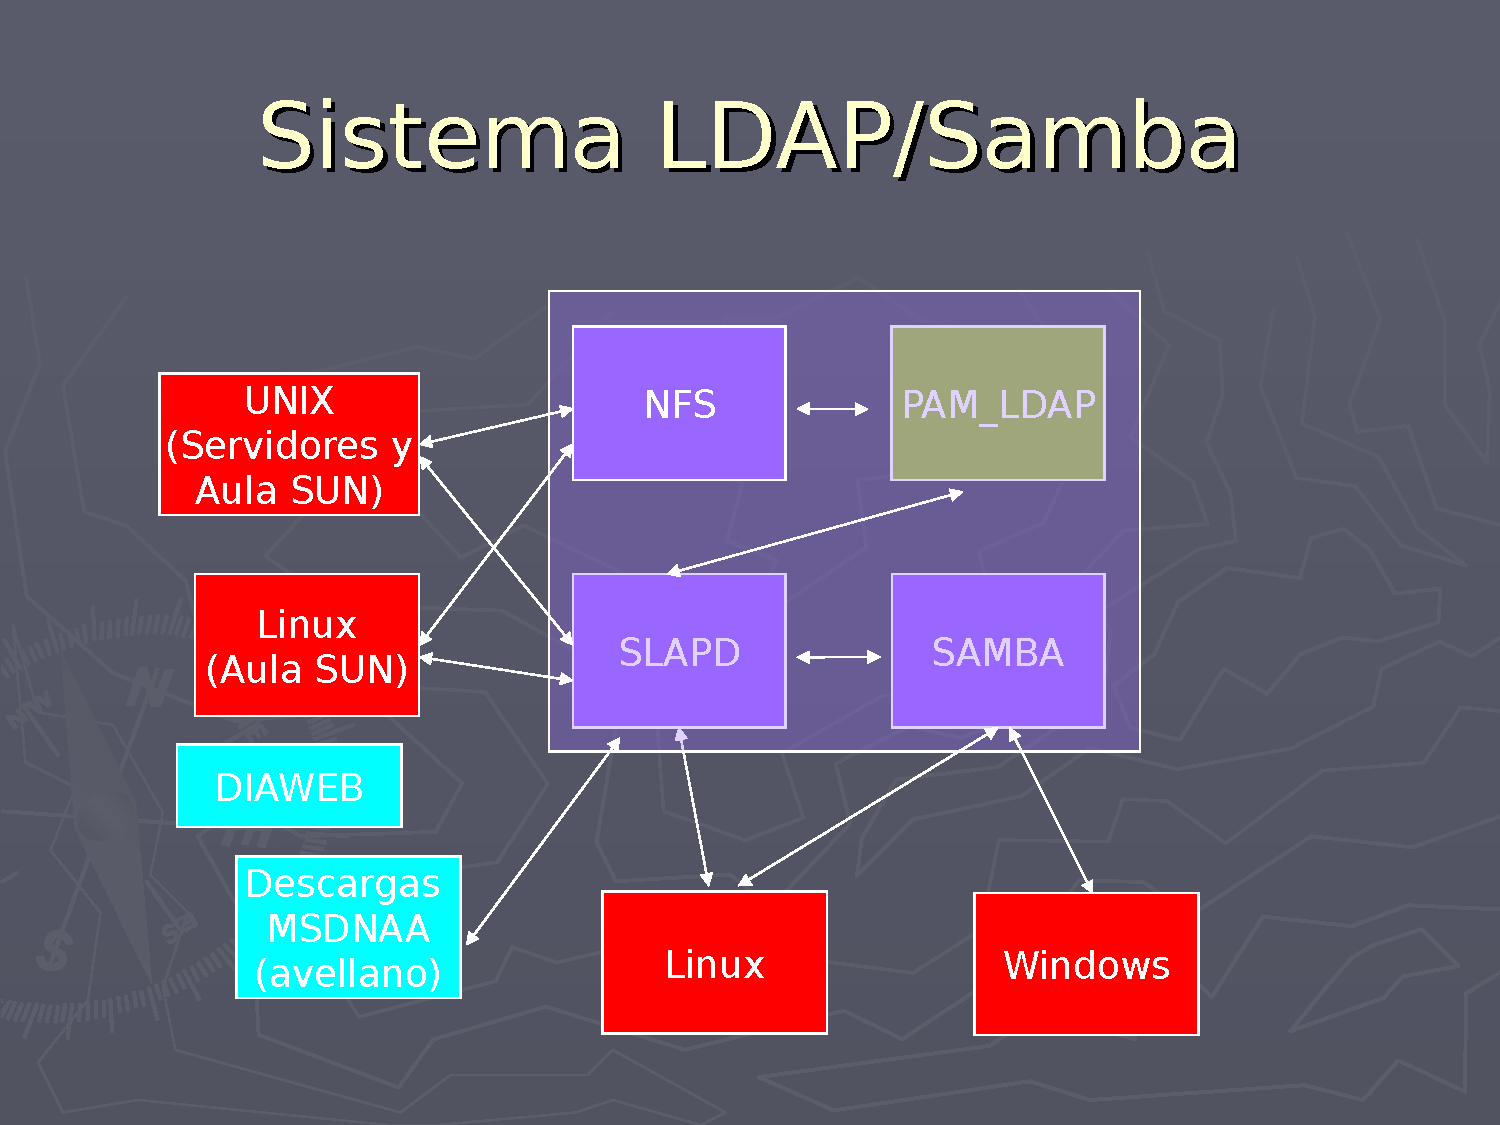
\includegraphics[width=0.7\textwidth]{Chapter6/Figures/LDAP.pdf}
	\caption[Esquema de los componentes del sistema de autenticación y gestión de archivos]{Esquema de los diferentes componentes del sistema de autenticación y gestión de archivos, así como de una serie de componentes adicionales. Obsérvese la interacción entre los componentes situados en el rectángulo interior}
	\label{fig:arquitectura_ldap}
\end{figure}

\subsection{Características en detalle}

Debido a la heterogeneidad de los diferentes equipos presentes en la infraestructura, el sistema debe posibilitar el acceso a todos los equipos utilizando el mismo conjunto de credenciales. Esto implica que el sistema debe ser compatible con al menos los sistemas operativos GNU/Linux, Microsoft Windows y Solaris. Por ello se interconecta el servidor LDAP con Samba, así como el PAM (\textit{Pluggable Authentication Module}) tanto en el cliente como el servidor.

Sin embargo el sistema permite también que los usuarios puedan almacenar información en un espacio centralizado al que es posible acceder desde cualquier equipo, facilitando la copia de ficheros entre nodos, uniformidad de los diferentes equipos. Esto se consigue utilizando un servidor NFS (\textit{Network File Storage}).

\subsection{Utilización en el sistema}

En el sistema se aprovechará principalmente la funcionalidad de autenticación provista por el servidor LDAP, debido a que uno de los objetivos principales del sistema es evitar ``cuellos de botella'' debido al uso de un servidor de almacenamiento central. Se facilitará la replicación de servicios con herramientas creadas a tal efecto (ver \ref{marcodiscover}) en su lugar.%TODO En cualquier caso, se plantea permitir el acceso al NFS desde el sistema como complemento, pero no como espacio principal de almacenamiento.

El sistema aprovecha el módulo PAM para realizar el proceso de autenticación.

\subsubsection{pam\_mkhomedir}
\label{pam_mkpolohomedir}

\textbf{PAM} permite ampliar la funcionalidad que ofrece por defecto mediante la inclusión de \textit{módulos}, pequeñas bibliotecas compartidas de código con las acciones a realizar.

Uno de los módulos incluidos en la instalación por defecto de \textbf{PAM} es \textbf{mkhomedir}, encargado de la creación de un directorio propio para el usuario en caso de que aún no se haya realizado dicha acción. El proceso consiste en una copia del directorio \textbf{skeleton} (generalmente situado en \texttt{/etc/skel}) y la correcta fijación de permisos en el mismo.

Sin embargo, el directorio únicamente es creado en el nodo al que se accede. La filosofía del sistema implica la creación de un sistema que se componga de varias unidades, pero se comporten como una única entidad, por lo que obligar al usuario a acceder a todos los nodos para poder trabajar en el sistema completo anula dicha transparencia. Es necesario contar con un sistema que extienda la funcionalidad de \texttt{mkhomedir} para incluir el resto de nodos en la creación del directorio.

Con este objetivo nace \texttt{pam\_mkpolopohomedir}, un módulo basado en \texttt{mkhomedir} que hace uso de \textbf{MarcoPolo} para detectar los nodos presentes en la red que ofrezcan el servicio \texttt{polousers} y solicitar a los mismos la creación del directorio de inicio.

El módulo se implementa en C debido a que es el lenguaje con el que los módulos de PAM se construyen por defecto y utiliza por tanto el \textit{binding} de MarcoPolo para este lenguaje. Existen sin embargo herramientas para desarrollar el mismo en Python\footnote{\href{http://pam-python.sourceforge.net/}{http://pam-python.sourceforge.net}}.

%TODO: Mover al catálogo técnico del módulo
% Un módulo en PAM debe implementar una serie de funciones que constituirán los puntos de entrada al módulo\citationneeded{pam manpages}:

% \begin{itemize}
% \item \texttt{PAM\_EXTERN int pam\_sm\_open\_session(pam\_handle\_t \* pamh, int flags, int argc ,const char **argv)}\\

% Es la función que \textbf{PAM} invoca al incluir el módulo. Incluye en el mismo una estructura \texttt{pam\_handle\_t} con toda la información relevante sobre el usuario que ha iniciado sesión y los parámetros indicados en los ficheros de configuración de \texttt{PAM} (en el caso de este módulo, los permisos del directorio de inicio y la localización del directorio \textit{skeleton}). 

% %comoPpunto de entrada al móduloal inicialmente

% \item \texttt{PAM\_EXTERN int pam\_sm\_close\_session(pam\_handle\_t * pamh, int flags, int argc, const char **argv)}

% Es la función que \textbf{PAM} utiliza para indicar al módulo que la sesión ha terminado. En el caso del módulo a crear no se debe realizar ninguna acción en este evento, sin embargo es necesario implementarla debido a que PAM la requiere.

% \item \texttt{struct pam\_module \_pam\_mkhomedir\_modstruct}

% Define las características del módulo y los puntos de entrada que define.
% \end{itemize}

El módulo realiza la siguiente secuencia de pasos:

\begin{enumerate}
	\item Determina la información de interés a partir de los datos provistos por \textbf{PAM} y las acciones a llevar a cabo. En caso de que el directorio ya exista, se omite la creación del mismo y únicamente se solicita la creación en el resto de nodos\footnote{Este paso siempre es necesario para facilitar la expansibilidad del sistema: añadir un nuevo nodo tras la creación del directorio en el resto haría que este no fuera accesible de no ser por la repetición de este paso}.
	
	\item Realiza si es necesaria la creación del directorio en el nodo actual.
	
	\item Detecta con \textbf{MarcoPolo} el resto de nodos dispuestos a colaborar en el sistema (aquellos que oferten el servicio \textbf{polousers}).
	
	\item Solicita a cada uno de ellos la creación del directorio.
	
	\item Una vez que todos los nodos han realizado la acción solicitada, se da acceso al sistema.
\end{enumerate}

Todas las operaciones realizan escrituras en ficheros de \textbf{log} para su posterior análisis.

%%TODO: definir en detalle
En cada uno de los nodos exisitirá por tanto una instancia del servicio \textbf{polousers} que se encargará de procesar las peticiones.

\paragraph{Seguridad\\}

Al tratarse de acciones llevadas a cabo por usuarios con privilegios elevados y que involucran la gestión de información personal, todas las comunicaciones se realizan utilizando conexiones cifradas mediante \textit{sockets} \textbf{TLS} (\textit{Transport Layer Security}) con certificados en ambos lados de la conexión, que son verificados por el contrario (ver \ref{teoria:autenticacionmutua}).

\paragraph{Extensibilidad\\}

El módulo ha sido diseñado con el objetivo de posibilitar la adición de nueva funcionalidad al mismo. Únicamente es necesario definir las acciones a llevar a cabo en el servicio \textbf{polousers} y solicitar su realización mediante la sintaxis de comandos de \textbf{MarcoPolo}.

%%%

%%%%%%%%%%%%%%%%%%%%%%

\subsection{MarcoPolo}

Sumada a las herramientas creadas en el sistema, es necesario llevar a cabo una serie de operaciones que posibiliten el acceso a servicios más básicos tales como la autenticación de los usuarios del sistema, %TODO etc

Con el objetivo de mejorar la situación actual en la infraestructura a analizar, se tratan los siguientes problemas.

\section{Instalación del sistema}

El sistema a crear requiere de la instalación de diferentes componentes, en particular el sistema operativo, antes de poder ser utilizado. Dicha instalación, si es realizada en cada nodo secuencialmente, implica una gran carga de trabajo y aumenta la propensión a errores durante dicho proceso (en particular si en el mismo existe una gran carga de trabajo que debe ser supervisado por un administrador humano). Una solución a este problema es la autoinstalación del sistema operativo partiendo de una imagen definida y probada por el administrador, que se cargará e instalará en cada nodo sin supervisión.

Una de las herramientas ya existentes para solucionar este problema es el \textbf{PXE} (\textit{Preboox eXecution Environment})\cite{pxeintel}, un estándar \textit{de facto}\cite{avramov:architecture} para la carga de un sistema operativo desde un servidor. El estándar se apoya en protocolos presentes en la práctica totalidad de sistemas, tales como \textbf{DHCP}, \textbf{TFTP} y \textbf{TCP/IP}. El descubrimiento de servicios se realiza mediante una extensión en el mensaje \textbf{DHCPDISCOVER} que envía el servicio \textbf{DHCP} en su secuencia de arranque\cite{rfc4578}. El servidor \textbf{DHCP}, si implementa esta extensión del protocolo, enviará la información sobre la localización de cada uno de los servidores de arranque al cliente, que procederá a la descarga utilizando el protocolo \textbf{TFTP} y posterior instalación\cite{pxeoverview}.

Sin embargo, el uso de este protocolo requiere un controlador de interfaz de red (\textbf{NIC}) en el cliente que soporte el protocolo \textbf{PXE}. Generalmente dicho controlador se incluye como extensión de la \textbf{BIOS} o en equipos más modernos como código \textbf{UEFI}. La \textbf{Raspberry Pi} carece de este tipo de \textit{software}, pues delega todo el arranque del sistema a los datos presentes en la tarjeta SD, y por tanto no es posible realizar ningún tipo de arranque en red sin la previa instalación de un conjunto de aplicaciones que realicen la descarga del sistema operativo. Es por ello que el uso de \textbf{PXE} como herramienta de arranque debe ser desestimado.

\subsection{marco-netinst}

Debido a la falta de soporte para \textbf{PXE} u otra alternativa similar, es necesario crear una herramienta que se encargue de la detección de un servidor que aloje la imagen del sistema operativo, la descarga del mismo y su instalación. Con este objetivo se crea la herramienta \textbf{marco-netinst}.

\textbf{marco-netinst} es una ramificación del proyecto \textbf{rasbpian-ua-netinst}\cite{raspbian-ua-netinst}. Esta utilidad permite instalar un conjunto mínimo de utilidades que posibilitan la descarga de un sistema operativo desde los repositorios de \textbf{Debian} y su instalación. La ramificación incluye las siguientes modificaciones:

\begin{itemize}
	\item Instalación de \textbf{ArchLinux ARM} en lugar de \textbf{Raspbian}.
	\item Instalación del sistema operativo completo a partir de un archivo \textbf{.tar.gz} en lugar de la descarga de paquetes\footnote{\textbf{raspbian-ua-netinst} utiliza el paquete cdebootstrap-static para la descarga e instalación de todos los archivos. Existe una herramienta para ArchLinux similar, denominada \textbf{Archbootstrap}\\
	\href{https://wiki.archlinux.org/index.php/Archbootstrap}{https://wiki.archlinux.org/index.php/Archbootstrap}\\
	\href{https://packages.debian.org/sid/cdebootstrap-static}{https://packages.debian.org/sid/cdebootstrap-static}}.
	\item Nuevo \textit{script} de carga del \textit{software} en la tarjeta SD (en el paquete original se delega a utilidades de terceros).
	%TODO\item Posibilidad de aplicar diferentes esquemas de particionado
	\item Detección del servidor sin configuración previa utilizando \textbf{MarcoPolo}.
	%TODO\item Interfaz administrativa de los sistemas operativos ofrecidos
\end{itemize}

La especificación en detalle del funcionamiento de la herramienta se detalla en el anexo%TODOf






La complejidad que acarrea el uso de aplicaciones distribuidas hace necesario el uso de herramientas que permitan el desarrollo de forma cómoda del propio sistema, su uso posterior como herramienta de prueba de aplicaciones distribuidas y por último, facilitar el aprendizaje de algoritmos y herramientas distribuidas.

Muchas de las aplicaciones distribuidas utilizadas incluyen varias herramientas para facilitar su uso. Sin embargo estas soluciones suelen ser diseñadas para el propósito específico de dicha aplicación, y son difíciles de adaptar a otros contextos. Debido a esta carencia, se han creado varias herramientas propias que permiten aprovechar al máximo este sistema.


\subsection{rsyslog}

\section{Bibliotecas}

\subsection{quick2wire-cpp-api}

Uno de los periféricos de interés en el desarrollo del sistema es el puerto \textbf{GPIO} \textit{General Purpose Input-Output} presente en la Raspberry Pi. Dicho puerto permite a los usuarios del sistema analizar de forma visual el comportamiento de una aplicación distribuida, ser utilizado como indicador del estado de la máquina, etcétera.

El funcionamiento del puerto presenta un problema para el desarrollo del proyecto. El acceso al hardware se consigue mediante el acceso a una serie de direcciones de memoria sobre las que se definen diferentes valores (dirección de cada uno de los pines, valor, etcétera). Dichas direcciones de memoria se definen en el fichero \texttt{/dev/mem}, que representa la memoria física presente en todo el nodo, así como este tipo de periféricos.

Debido al riesgo que conlleva el acceso a este dispositivo por cualquier usuario, únicamente el superusuario tiene permisos para manipular el mismo (poder modificar este fichero implica ganar control absoluto sobre la memoria del sistema). Esto implica que el acceso al puerto \textbf{GPIO} está restringido al superusuario o alguien con permisos para acceder al mismo (mediante la herramienta \texttt{sudo}).

Quedando descartada la opción de elevar los privilegios de todos los usuario para que puedan hacer uso del puerto, es necesario buscar alternativas. Se busca una solución más eficaz que otorgar permisos de forma temporal o mediante supervisión de un administrador.

Tras la revisión de las diferentes alternativas de terceros existentes que proporcionan el acceso al puerto GPIO, \textbf{wiringPi2}\footnote{\citationneeded}, \textbf{RPi.GPIO}\footnote{\citationneeded} y \textbf{quick2wire}\footnote{\citationneeded}, únicamente esta última implementa un mecanismo que permite a los usuarios utilizar el puerto GPIO sin permisos. Por desgracia, esta biblioteca está implementada únicamente en Python, y el uso del puerto en el sistema está inicialmente planteado para el uso en aplicaciones creadas en C/C++ debido a que son los lenguajes utilizados en la asignatura \textbf{Arquitectura de Computadores}. Se valora la posibilidad de crear una traducción de la biblioteca quick2wire-python-api a C/C++, y dicha propuesta es admitida como camino de solución tras un prototipo inicial.

\subsubsection{Funcionamiento}

La biblioteca original aprovecha otro producto de \textbf{quick2wire}, la aplicación \textbf{gpio-admin}. Escrita en C, dicha aplicación permite realizar operaciones sobre las direcciones de memoria que se corresponden con el puerto \textbf{GPIO}. Mediante el uso de del bit de usuario \citationneeded{revisar} es posible hacer que el usuario ejecutor sea a efectos de acceso a \texttt{/dev/mem} el superusuario. Este sistema es similar al de la herramienta \textbf{passwd}.

La herramienta establece una correspondencia (\textit{``mapping''}) entre las direcciones asociadas al GPIO y un directorio virtual en \texttt{/sys/class/gpio}\footnote{En la biblioteca original, escrita para Raspbian, la correspondencia se realizaba con \texttt{}\citationneeded{Buscar}. Se ha modificado el código para posibilitar la compatibilidad con Arch Linux}.

Posteriormente es necesario únicamente utilizar esta herramienta mediante llamadas al sistema a través de la biblioteca. Es por ello que \textbf{quick2wire-cpp-api} (y la implementación original en Python) pueden considerarse wrappers de esta utilidas, aportando poca funcionalidad más allá de una capa de abstracción.

\subsubsection{Descripción del código}

La biblioteca es compatible con C y C++ ofreciendo un conjunto de llamadas similares a la implementación original en Python. Sólo se ha implementado aquella funcionalidad necesaria para posibiltar el acceso a los pines GPIO (y actualmente únicamente en modo salida) %TODO hacer GPIO in

La interfaz con I\textsuperscript{2}C y SPI aún no está implementada.